\documentclass[12pt,a4paper]{article}
% Preámbulo del informe de la Etapa 4: el de la Etapa 3. Computer Modern a 12pt,
% como los documentos de la cátedra, y todo en negro.
\usepackage[T1]{fontenc}
\usepackage[utf8]{inputenc}
\usepackage{lmodern}
\usepackage{amsmath,amssymb}
\usepackage[spanish,es-noquoting,es-noshorthands,es-tabla]{babel}
\usepackage[a4paper,margin=2.6cm,headsep=14pt]{geometry}
\usepackage{microtype}
\usepackage{booktabs}
\usepackage{longtable}
\usepackage{array}
\usepackage{xcolor}
\usepackage{fancyhdr}
\usepackage{titlesec}
\usepackage{enumitem}
\usepackage{fancyvrb}
\usepackage[hidelinks,bookmarks=true]{hyperref}

\usepackage{float}
\usepackage{graphicx}
\usepackage{pdflscape}
\DeclareUnicodeCharacter{2014}{---}
\DeclareUnicodeCharacter{2026}{\ldots}

% --- Paleta ------------------------------------------------------------------
\definecolor{tinta}{rgb}{0,0,0}

\color{tinta}

% --- Títulos ------------------------------------------------------------------
\titleformat{\section}{\Large\bfseries\color{tinta}}{\thesection}{0.7em}{}
\titleformat{\subsection}{\large\bfseries\color{tinta}}{\thesubsection}{0.7em}{}
\titleformat{\subsubsection}{\bfseries\color{tinta}}{\thesubsubsection}{0.7em}{}
\titlespacing*{\section}{0pt}{2.4ex plus 1ex minus .2ex}{1.3ex plus .2ex}

% --- Encabezado y pie ---------------------------------------------------------
\setlength{\headheight}{14pt}
\pagestyle{fancy}
\fancyhf{}
\renewcommand{\headrulewidth}{0.4pt}
\renewcommand{\headrule}{\hbox to\headwidth{\color{tinta}\leaders\hrule height \headrulewidth\hfill}}
\fancyhead[L]{\footnotesize\color{tinta}Compiladores e Intérpretes — Etapa 4}
\fancyhead[R]{\footnotesize\color{tinta}\nouppercase{\leftmark}}
\fancyfoot[C]{\footnotesize\color{tinta}\thepage}

% --- Bloques de consola --------------------------------------------------------
% \footnotesize y no \small: la línea más larga de una sesión de consola tiene
% 82 caracteres y a \small no entra en la caja de texto.
\DefineVerbatimEnvironment{consola}{Verbatim}%
  {fontsize=\footnotesize,xleftmargin=1.1em,formatcom=\color{tinta}}

\setlength{\emergencystretch}{4.5em}
\tolerance=3000

\setlist[itemize]{leftmargin=1.3em,itemsep=0.25ex,topsep=0.5ex}
\setlist[enumerate]{leftmargin=1.5em,itemsep=0.25ex,topsep=0.5ex}
\setlist[description]{leftmargin=1.3em,itemsep=0.35ex,topsep=0.6ex}
\renewcommand{\arraystretch}{1.25}

\usepackage{ragged2e}

\begin{document}

% ===========================================================================
% Portada
% ===========================================================================
\begin{titlepage}
\thispagestyle{empty}
\raggedright
\vspace*{2.2cm}

{\footnotesize\sffamily
UNIVERSIDAD NACIONAL DEL SUR\\
Departamento de Ciencias e Ingeniería de la Computación\\
Compiladores e Intérpretes --- Segundo Cuatrimestre de 2026\par}

\vspace{2.4cm}
{\rule{\textwidth}{0.6pt}}
\vspace{1.1cm}

{\Huge\bfseries Compilador de MiniJava\par}
\vspace{0.5cm}
{\LARGE\color{tinta} Etapa 4 --- Analizador Semántico II\\[0.25cm]
\large Árboles Sintácticos Abstractos y Chequeo de Sentencias\par}

\vspace{1.1cm}
{\rule{\textwidth}{0.6pt}}

\vspace{2.6cm}
{\large Agustín Paul\par}
\vspace{0.2cm}
{\normalsize L.U. 147524\par}
\vspace{0.4cm}
{Informe de entrega\par}

\vfill
{\color{tinta}\footnotesize \today\par}
\end{titlepage}

\thispagestyle{empty}
\tableofcontents
\newpage
\setcounter{page}{1}
\RaggedRight

% ===========================================================================
\section{Cómo compilar y ejecutar}
% ===========================================================================

Proyecto Maven con Java~25. Desde la carpeta \texttt{compilador/}:

\begin{consola}
$ mvn package          # compila, corre la suite y arma target/Compilador.jar
$ java -jar target/Compilador.jar programa1.java
Compilacion Exitosa

[SinErrores]
\end{consola}

El fuente es el único argumento y puede tener cualquier extensión. Sin opciones corre esta etapa,
que también se elige con \texttt{-{}-etapa=4}. Las etapas anteriores siguen disponibles:
\texttt{-{}-etapa=1} corre sólo el léxico, \texttt{-{}-etapa=2} sólo el sintáctico y
\texttt{-{}-etapa=3} el chequeo de declaraciones, sin mirar los cuerpos.

% ===========================================================================
\section{Los árboles sintácticos abstractos}
% ===========================================================================

El sintáctico arma el AST de cada cuerpo con las acciones de un esquema de traducción sobre su
gramática LL(1), y lo cuelga del método o constructor de la tabla de símbolos. Los tipos de nodo
salen de la gramática original de la cátedra: cada sentencia y cada expresión con significado es
una clase. Si las declaraciones están bien y la tabla está consolidada, cada clase chequea el
cuerpo de los constructores y métodos que ella declara: cada nodo controla lo suyo y delega en sus
hijos. Una expresión devuelve su tipo, y calcula aparte si es un destino asignable o una llamada.
El primer error semántico termina el análisis.

\medskip
Los diagramas de clases (figuras~\ref{fig:sentencias} a~\ref{fig:contexto}) muestran todos los
campos, constructores y métodos del código. Lo subrayado es estático y lo que está en cursiva,
abstracto. Una referencia a otra clase dibujada es una relación, rotulada con el nombre del campo y
su multiplicidad (\texttt{0..1} si puede faltar, \texttt{*} si es una colección, ninguna si es
exactamente una), y una caja sin miembros se detalla en otro diagrama.

\begin{landscape}
\begin{figure}[H]
\centering
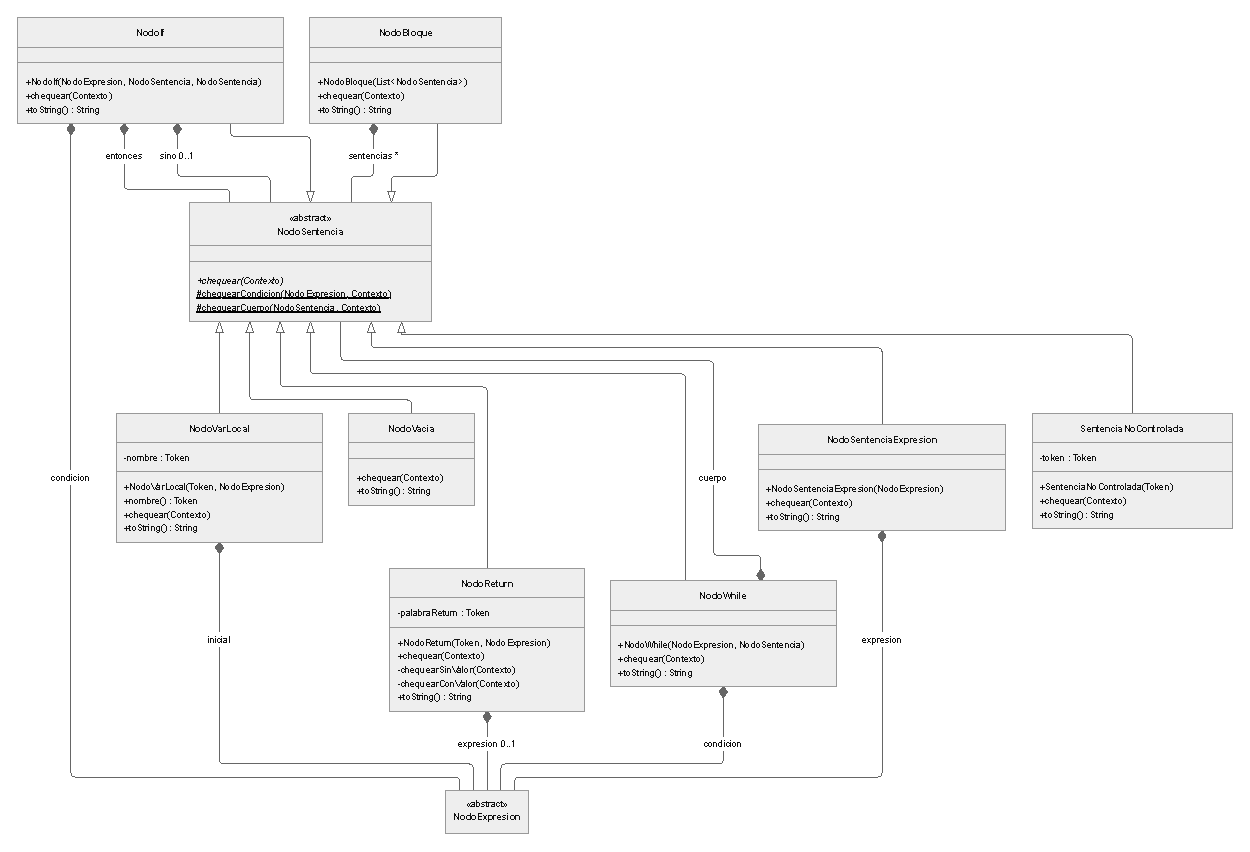
\includegraphics[width=\linewidth,height=0.86\textheight,keepaspectratio]{generado/sentencias.pdf}
\caption{Las sentencias. \texttt{NodoBloque} es el cuerpo de cada método y constructor.}
\label{fig:sentencias}
\end{figure}
\end{landscape}

\begin{landscape}
\begin{figure}[H]
\centering
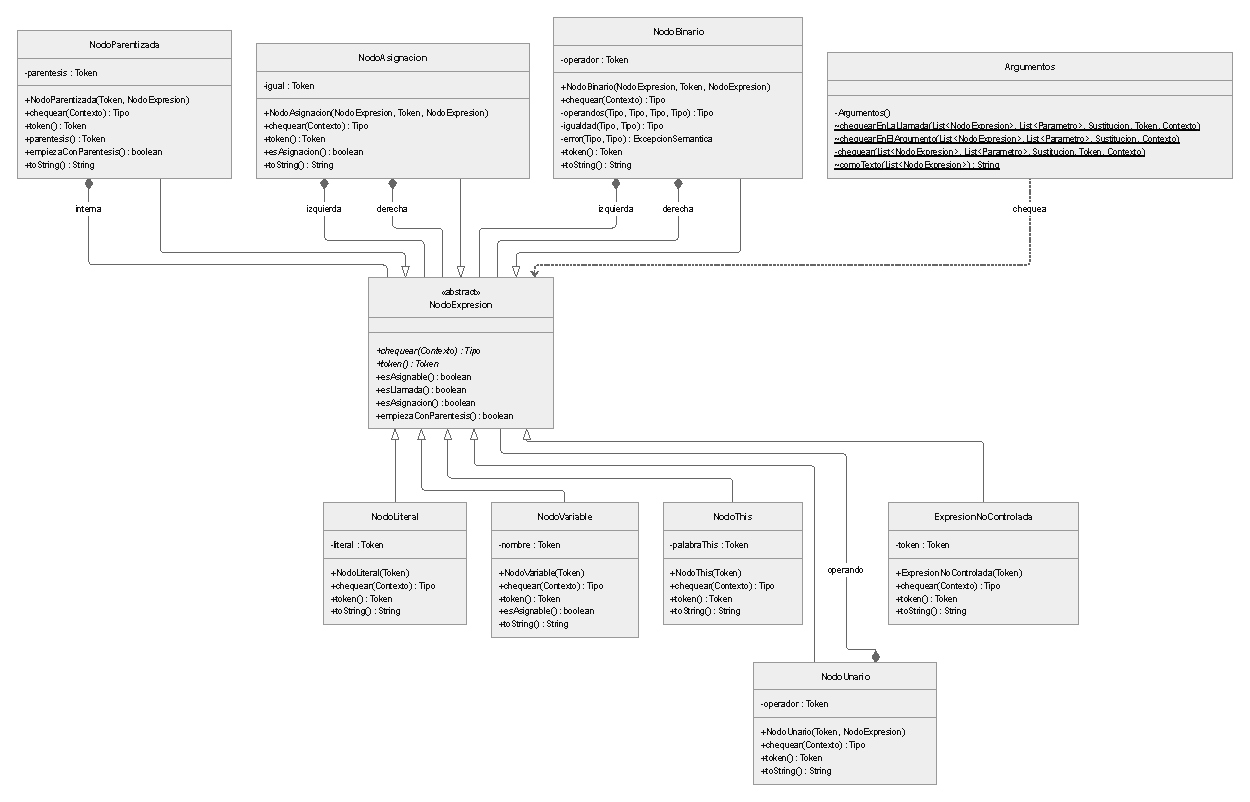
\includegraphics[width=\linewidth,height=0.86\textheight,keepaspectratio]{generado/expresiones.pdf}
\caption{Las expresiones. \texttt{token()} es el token donde se reporta un error de la expresión
entera.}
\label{fig:expresiones}
\end{figure}
\end{landscape}

\begin{landscape}
\begin{figure}[H]
\centering
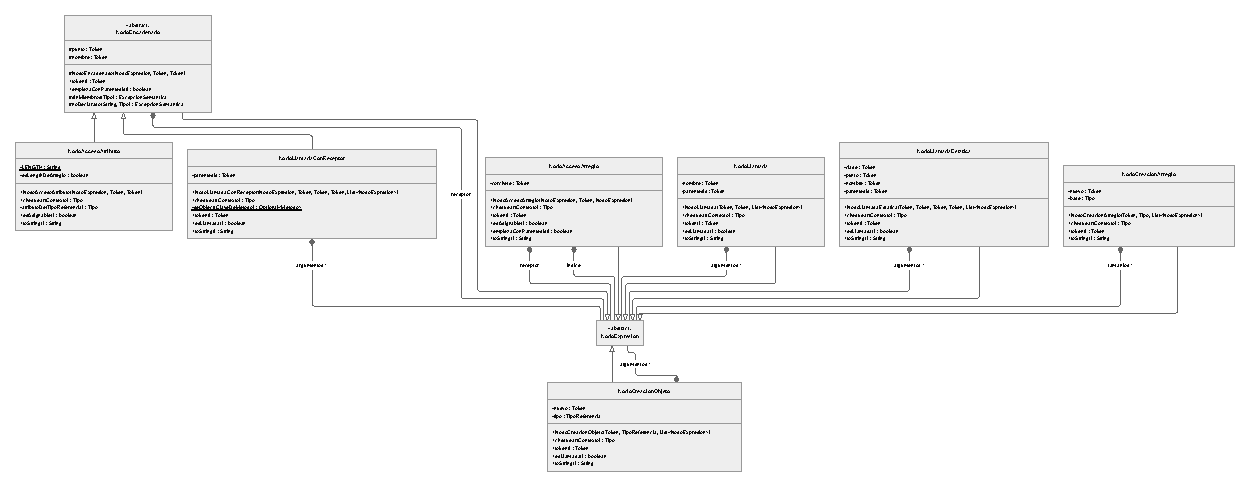
\includegraphics[width=\linewidth,height=0.86\textheight,keepaspectratio]{generado/llamadas-y-accesos.pdf}
\caption{Las llamadas, los accesos y las creaciones. Un encadenado guarda su receptor:
\texttt{a.b.m()} es la llamada a \texttt{m} sobre el acceso a \texttt{b} sobre \texttt{a}.}
\label{fig:llamadas-y-accesos}
\end{figure}
\end{landscape}

\begin{figure}[H]
\centering
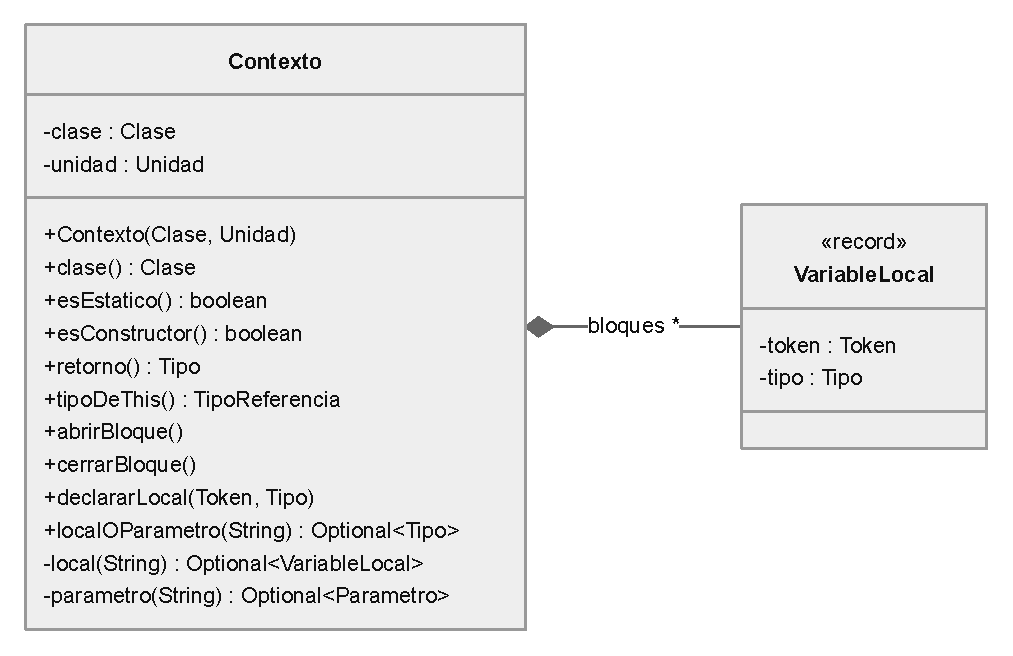
\includegraphics[width=0.7\textwidth]{generado/contexto.pdf}
\caption{El contexto del chequeo de una unidad: la clase, la unidad y las variables locales
visibles, un mapa por bloque abierto.}
\label{fig:contexto}
\end{figure}

% ===========================================================================
\section{Logros}
% ===========================================================================

Se intentan los logros que no requieren código:

\begin{itemize}
  \item \textbf{Imbatibilidad Semántica II}. Los casos de la cátedra dan el código exacto, y el
        corpus propio cubre cada control con casos con error y sin él.
  \item \textbf{Entrega Anticipada}.
  \item \textbf{Grandioso Laburo!}
\end{itemize}

\end{document}
